% Quantum Communication

\chapter{Quantum Communication Systems with non-Gaussian States}
    Thanks to quantum mechanics, it will be possible to overcome the limits of classical 
    communication systems. In the last decades the research in this field has led to very 
    intresting results that could significantly improve the performance of communication systems. 
    This chapter gives a brief overview of quantum communication tools: in the first section we
    give an overview of a quantum communication system, in the second we present the equivalents 
    of classical modulation for quantum communication systems; in the last 
    section we report the concept of quantum states discriminator (QSD), included when it can be 
    considered optimal.

    \section{Quantum Communication System}
    \begin{figure}[t]
        \begin{center}
            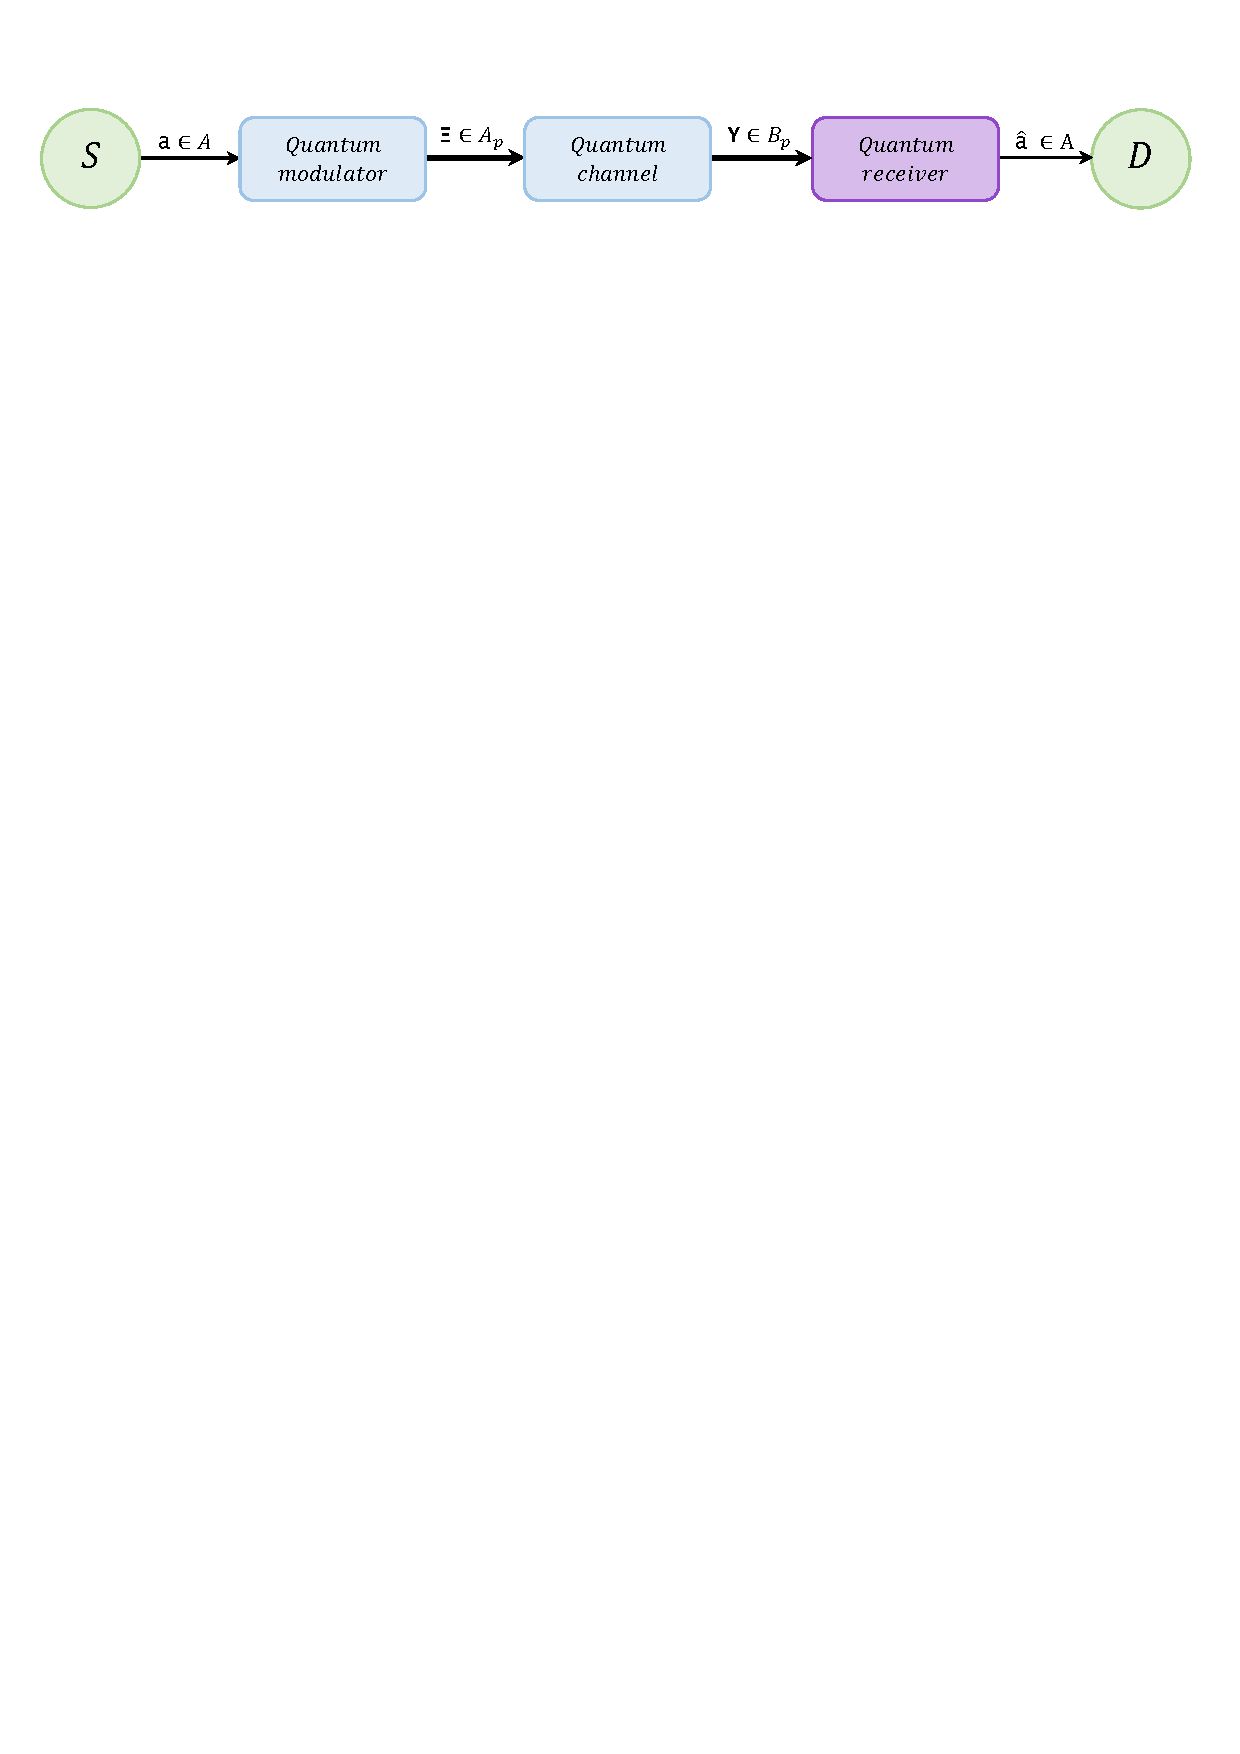
\includegraphics[width=1\textwidth]{fig3.0.pdf}
            \caption{Block-chain of a quantum communication system}
            \label{fig:3.0}
        \end{center}
    \end{figure}
    A quantum communication system can be described similarly to a classical one, as we can 
    see in figure \ref{fig:3.0}. An information source emits a flow symbols $a \in \mathcal{A}$, this
    can be considered, without loss of generality, as a flow of bits. These bits have to be 
    modulated with a quantum modulator that emits on the communication channel a quantum state
    $\Operator{\varXi} \in \mathcal{A}_p$ for each bit or group of bits. The channel can distort the
    state and deliver the state $\Operator{\varUpsilon} \in \mathcal{B}_p$ that is in general 
    different from $\Operator{\varXi}$.
    The receiver have to recognize the information $\hat{a}$ as well as possible, i.e. with 
    the minimum possible error probability.

    \section{Quantum Modulation}
    As in a classical system, it is possible to define the concept of modulation for a 
    quantum communication system. The transmitted information will be associated to a 
    quantum state of the electromagnetic field, so it can be transmitted on the communication 
    channel.

    \begin{figure}[tbp]
        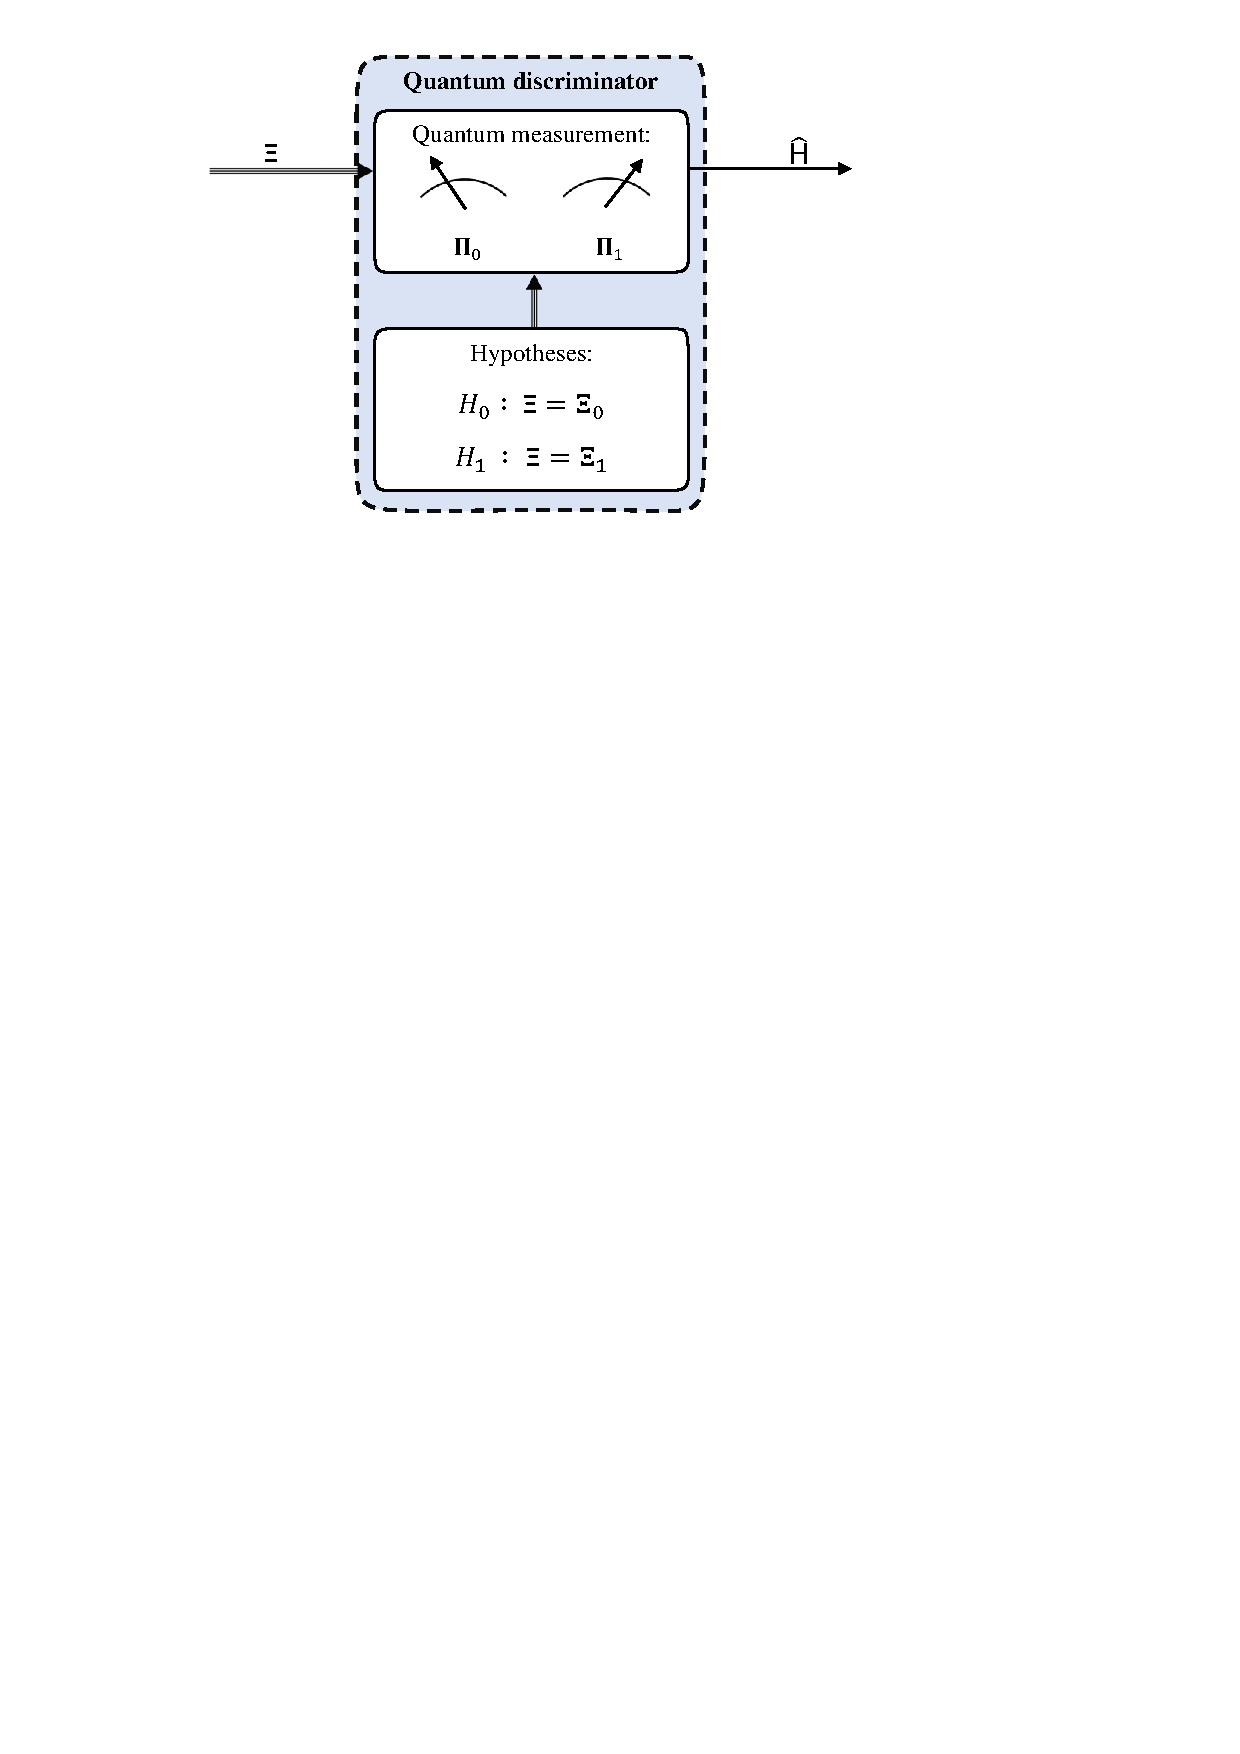
\includegraphics[width=1\textwidth]{fig2.1.pdf}
        \caption{Block diagram of a quantum transmitter.}
        \label{fig:2.1}
    \end{figure}
    It is possible to think about the quantum transmitter as in figure \ref{fig:2.1}. The bit source
    emits a bit sequence $a[n]$, the serial-parallel converter parallelizes a group of $l$-bit (where
    if $L$ is the number of quantum states, $l=\log_2(L)$) and sends them to the quantum modulator.
    This latter associates one quantum state to every group of bit. The operation of quantum state 
    creation, in real cases, is affected by noise.

    The sequence of operations is very close to a classical transmitter: the main difference is that
    the modulator maps the bits into quantum states instead of classical modulation. Therefore, it is 
    possible to achieve the quantum equivalent of classical modulation, with several states. After 
    that, the impact on performance can be tested.
    This thesis only considers and assesses the binary cases, in the OOK and BPSK 
    configuration.
    
    \subsection{OOK modulation}
        The OOK (on-off keying) is the most simple possible configuration for a communication system.
        The quantum implementation of that is realized associating the low-energy state to the 
        ground state $\ket{0}$ and the high-energy state to another state. It is important to
        consider that the physical realization of these states are not free-noise; this issue will be
        considered using noisy states \ref{eq:2.1.1}.
        \begin{equation}
            \pmb{\Xi}_0 = \pmb{\Xi}_{th}
            \label{eq:2.1.1}
        \end{equation}
        \begin{equation*}
            \pmb{\Xi}_1 = \pmb{\Xi}_{th}(\mu)
        \end{equation*}
        In the equation \ref{eq:2.1.1}, the high-energy state is associated to a coherent state. This 
        configuration has been widely analyzed in \cite{helstrom1,helstrom2,coherentComm1,coherentComm2,
        coherentComm3,coherentComm4} but this is not the only possible way. The use of PACS states 
        $\pmb{\Xi}_{th}^{(k)}(\mu)$ is analyzed in \cite{PACSDisc,tesiGuerrini}; the use of PASS are briefly
        assessed in the following chapter of this thesis.

    \subsection{BPSK modulation}
        BPSK quantum systems are implemented using two states with opposite amplitude, like
        \begin{equation}
            \pmb{\Xi}_0 = \pmb{\Xi}_{th}(-\mu)
            \label{eq:2.1.2}
        \end{equation}
        \begin{equation*}
            \pmb{\Xi}_1 = \pmb{\Xi}_{th}(\mu).
        \end{equation*}
        There is no guarantee that the use of a BPSK solution in  a quantum system will 
        improve its performance. The effect depends on which are the used states. In the next chapter some 
        configuration are assessed.

    \section{Quantum Discriminator}
    The problem of quantum state discrimination (QSD) is one of the most important
    aspects of quantum communication. As in classical communication, the ability to 
    distinguish between two or more states in presence of noise can be decisive in order to determine
    the performance of the communication system. However, differently from the classical situation,
    the discrimination can be done using a custom-designed quantum discriminator, overcoming
    the classical physics limits.

    \subsection{Binary quantum state discrimination}
    \begin{figure}[ht]
        \begin{center}
            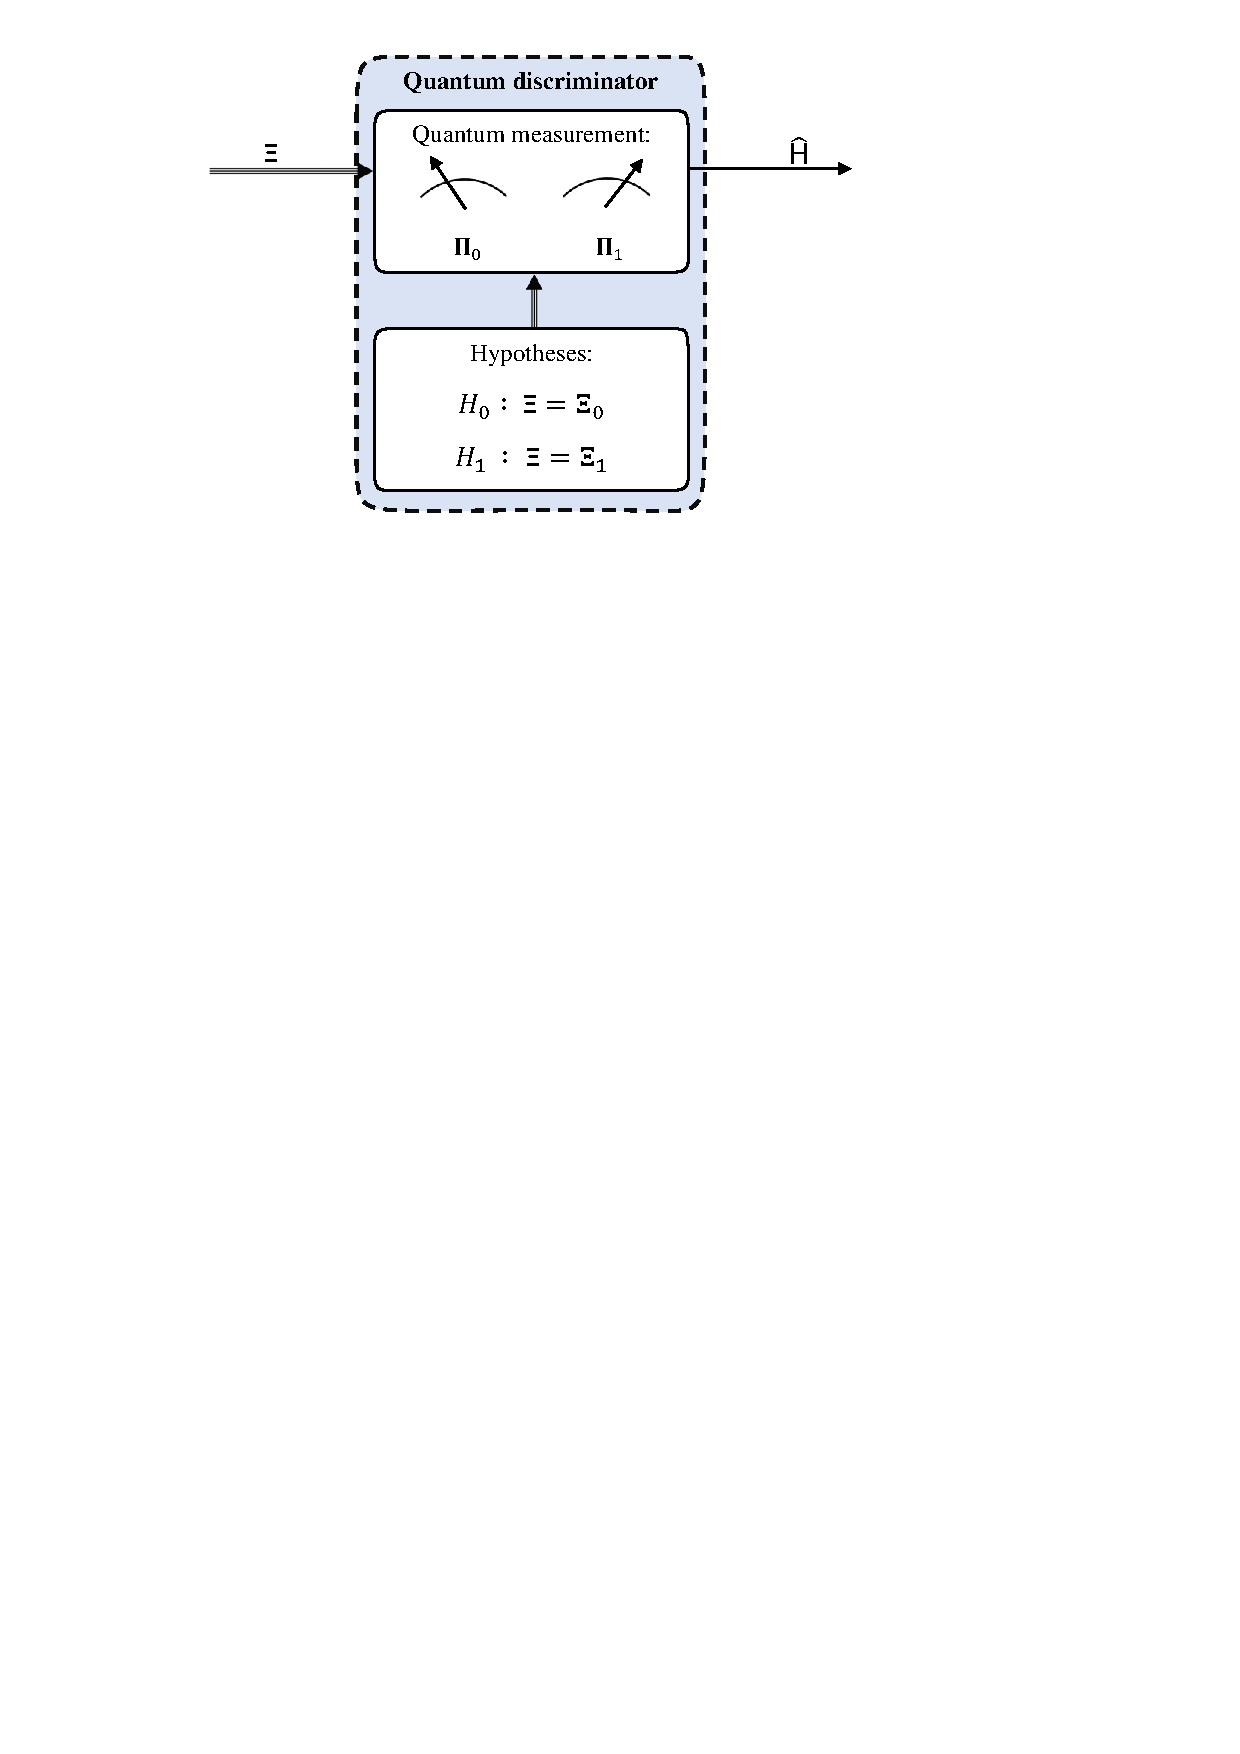
\includegraphics[width=0.75\textwidth]{fig2.2.pdf}
            \caption{Binary quantum state discriminator.}
            \label{fig:2.2}
        \end{center}
    \end{figure}
    The problem of discrimination between two quantum states is realized, as every measurement
    process \ref{post:2}, using an operator or a set of operators.
    If the state of the system is unknown, as shown in figure \ref{fig:2.2}, there are two hypotheses
    about the state $\pmb{\Xi}$ (the problem is easly generalizable for $M$ different states),
    given by:
    \begin{equation}\begin{split}
        H_0 : \pmb{\Xi}=\pmb{\Xi}_0\\
        H_1 : \pmb{\Xi}=\pmb{\Xi}_1
        \label{eq:binHyp}
    \end{split}\end{equation}
    It is necessary a set of two positive-definites operator (POVM)
    \begin{equation}
        \mathcal{P}=\{\pmb{\Pi}_0,\pmb{\Pi}_1\}
    \end{equation}
    for the discrimination process, and the probability that the hypothesis $H_j$ is choosen
    if $H_k$ is the right choose is given by \cite{tesiGuerrini}:
    \begin{equation}
        \mathbb{P}\{H_j|H_k\}=tr\{\pmb{\Xi}_k\pmb{\Pi}_j\}.
    \end{equation}
    The distribution error probability (DEP) in the discrimination process, if $p_0$ and $p_1$ are 
    respectively the probabilty of symbols $0$ and $1$, is so given by
    \begin{equation}
        P_e=1-\left(p_0 tr\{\pmb{\Xi}_0\pmb{\Pi}_0\}+p_1 tr\{\pmb{\Xi}_1\pmb{\Pi}_1\}\right).
    \end{equation}

    \subsection{Optimal discriminator}
    The issue of finding the optimal POVM that minimizes the DEP was exhaustively discuss  by Helstrom in 
    \cite{helstrom3,helstrom4}. The minimum distribution error probability (MDEP) for a binary 
    communication system is given by the well-known Helstrom bound
    \begin{equation}
        \breve{P}_e = \frac{1}{2} \left(1-\norm{p_1 \pmb{\Xi}_1 - p_0 \pmb{\Xi}_0}_1 \right),
        \label{eq:HelstromBound}
    \end{equation}
    where $p_0,\ p_1$ are the probability that the states $\pmb{\Xi}_0,\ \pmb{\Xi}_1$ are trasmitted
    and the operator $\norm{\cdot}_1$ represents the trace norm. 
    The MDEP \ref{eq:HelstromBound} is obtained with the following POVM:
    \begin{equation}
        \breve{\pmb{\Pi}}_0 = \sum_{\substack{i \\ \lambda_i<0}} \ket{\lambda_i}\bra{\lambda_i},
    \end{equation}
    \begin{equation*}
        \breve{\pmb{\Pi}}_1 = 1-\breve{\pmb{\Pi}}_0 = 
        \sum_{\substack{i \\ \lambda_i \geq 0}} \ket{\lambda_i}\bra{\lambda_i};
    \end{equation*}
    where $\ket{\lambda_i}$ is the eigenvector of $p_1 \pmb{\Xi}_1 - p_0 \pmb{\Xi}_0$ associated to 
    the eigenvalue $\lambda_i$.
    For pure states, i.e $\pmb{\Xi}_0 = \ket{\psi_0}\bra{\psi_0}$ and $\pmb{\Xi}_1 = \ket{\psi_1}
    \bra{\psi_1}$, the equation \ref{eq:HelstromBound} begin
    \begin{equation}
        \breve{P}_e = \frac{1}{2} \left(1- \sqrt{1-4 p_0 p_1 \absolutevalue{\braket{\psi_0}{\psi_1}}^2}
        \right).
        \label{eq:HelstromBPure}
    \end{equation}
    It is possible to observe that, for pure states, the MDEP is equal to $0$ if $\braket{\psi_0}{\psi_1}$,
    that is $\ket{\psi_0}$ and $\ket{\psi_1}$ are orthogonal states.